\section{Surrogate Modeling \label{sec:SUMO}}

 A surrogate model, is an efficient mathematical model that represents the behavior of a complex system such as a circuit, software or wireless network. A surrogate model is trained at design time, using a limited number of input-output sample data points obtained through simulation or real-life experiments. It is especially suited for tasks with a large input space, as an accurate model can be trained based on relatively little input data points.
 
\begin{figure*}[t]
  \centering
  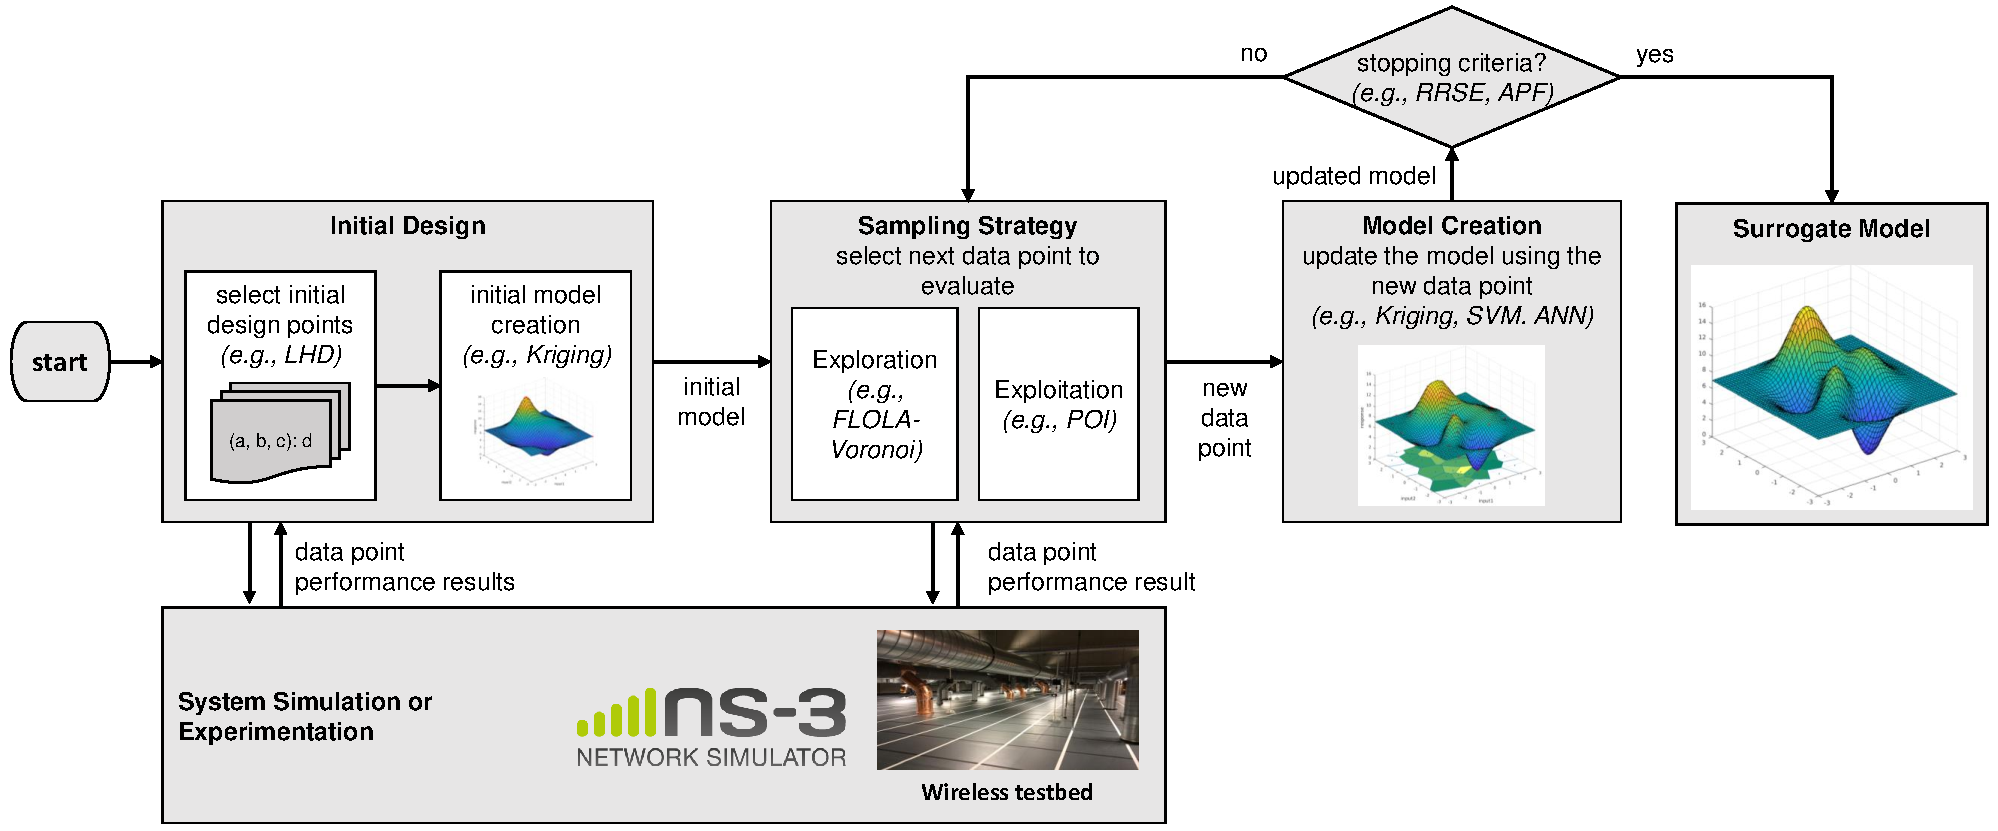
\includegraphics[width=0.9\textwidth]{figures/surrogate_modeling_approach}  \caption{surrogate modeling approach. \label{fig:surrogate_modeling}}
\end{figure*}

%  A simple example of a surrogate model is shown in Figure \ref{fig:sumo}, where the red dots correspond different input configuration settings, and the curve represents the predicted performance over the full design space. The output related to an input data point is generated using either real-life experiments, or via simulation software. 


% Traditionally, the one-shot approach is commonly used to train the model, in which the data points used for training are defined by generating an experimental design based on a space-filling criterion  at once. Because no prior information is available on the behaviour of the response surface it is hard to determine the size of a one-shot design, which is their major downside. 

% Sequential design turns this one-shot approach into an iterative process [3,24]. The acquired data and the constructed models from previous iterations are analyzed in order to intelligently select locations for new data points (sequential sampling). Next, the labels for these additional data points are obtained and new models can be trained or existing models can be updated.


% First of all this means there is no risk of over- or undersampling as the process can be halted when the desired ac- curacy is reached (or if the computational budget is exceeded). A second major advantage is that information provided by the con- secutive labels and intermediate models can guide the selection to obtain optimal locations for new data points. This allows the data distribution to be adapted and refined to the problem at hand as

 
%  Regression models describe the relationship between a response (output) variable, and one or more predictor (input) variables. The responses for new data can be predicted by using the trained model.

 
As illustrated in figure \ref{fig:surrogate_modeling},  surrogate modeling involves the following steps: (i) selecting initial data points to create a first simple model representation (initial design points), (ii) building an initial model with  the the selected initial design points, (iii) selecting the next sample data points to improve the  model if the model accuracy is not satisfactory, otherwise, terminating the modeling process. (iv) building an intermediary model with the previously collected design points, and going back to step (iii). The remainder of this section describes the method used in each steps in details.

 \subsection{Initial Design Points selection}
%However, the initial model requires a set of initial sample points from the design space and performance outputs.

% Before starting the sequential design approach, a coarse initial surrogate model is created based on a small set of data points. 
% To efficiently characterize the system using few design points, ideally space filling designs are used. %Ideally, space filling designs are used to optimally characterize the system behavior. 
% For example, Mehari \textit{et al.} compared several design point selection approaches \cite{SUMOWirelessConferencing}, with the \textit{Latin hypercube design} (LHD) \cite{viana2013} to be generally found the best performing. LHD is a stratified sampling method that selects sample points evenly along the configuration space while ensuring proportional representation of design variables. %Figure \ref{IllustrationSampling}b illustrates a surrogate model based on 20 initial samples using an LHD strategy.

The initial sample points have to be selected carefully to efficiently characterize the system. The existing sampling methods include \gls{lhd} \cite{viana2013}, Orthogonal sampling, Random sampling and  \textit{Hammersley Sequence Sampling} (HSS) \cite{wong1997sampling}. Among them, LHD has the best performance in general is the most commonly used approach, it selects sample points evenly along the configuration space while ensuring proportional representation of design variables. To obtain a better initial model, the number of initial sample points should be large, however, this increase the training time, therefore, a trade-off in terms of the initial design points is normally made. 

\subsection{(Initial) Surrogate Model Creation}

Based on the previously obtained data points, a surrogate model is created to predict how the performance metrics (i.e., output parameters such as throughput, latency or energy consumption) are influenced by the input parameters (i.e. the configuration settings). 

The surrogate model can be created using a variety of supervised machine learning and regression methods, such as Kriging \cite{forrester2008engineering}, polynomial response surfaces, radial basis functions, support vector machines (SVMs), space mapping, or artificial neural networks (ANNs). 


\begin{itemize}
    \item Support vector machines \textcolor{red}{todo}.
    \item  Linear regression, the relationships are modeled using linear predictor functions whose unknown model parameters are estimated from the data. \\
\begin{equation}
y_i = \beta_0 + \sum_{k=1}^{K} \beta_k f_k (X_{i1}, ..., X_{ip}) + \epsilon_i, i = 1, ..., n
\end{equation}
Where $f_k (.)$ is a scalar-valued function of the independent variables, $x_{ij}$,  might be in any form including nonlinear functions or polynomials. The response variable, $y_i$, is a linear function of the coefficients, $\beta_k$. The  noise terms, $\epsilon_i$ ((in contrast with the "signal" provided by the rest of the model)), are uncorrelated, and have independent and identical normal distributions with mean zero and constant variance, $\sigma^2$.
    \item  Gaussian process regression  models, also known as Kriging, are nonparametric kernel-based probabilistic models. A Gaussian prior is assumed for the regression curve, and the errors are assumed to have a multivariate normal distribution and the regression curve is estimated by its posterior mode. The Gaussian prior may depend on unknown hyperparameters, which are usually estimated via empirical Bayes. 
Kriging model are very popular in the modeling of  complex systems, including the complex wireless network \cite{SUMOWirelessConferencing,wowmom2018, LTEoptimization}.The kriging model is formed as:
\begin{equation}
\hat{f} (X) = \sum_{i=1}^{V} {a_i}{k(x, x_i)}
\end{equation}
Where $V$ is the amount of basis vectors, $x$ represent the input data vector and $k(x, x_i)$ is the kernel function. There are several kernel (covariance) functions used by kriging mode, such as, Squared Exponential Kernel, Exponential Kernel, Matern 3/2, Matern 5/2, Rational Quadratic Kernel. Among them, the Matern types of kernel functions are  widely used, and we use the Matern kernenl function with $v=3/2$ and $5/2$ is this paper. 
\end{itemize}

% Regression method: Kriging model, Gaussian Processes model, ... (explain all the ones we evaluate) \\


% ''constant": Model contains only a constant (intercept) term.\\
% ''linear": 	Model contains an intercept and linear terms for each predictor.\\
% "interactions'':	Model contains an intercept, linear terms, and all products of pairs of distinct predictors (no squared terms), considering the relationship among three or more variables, and describes a situation in which the simultaneous influence of two variables on a third is not additive.\\
% ''purequadratic":	 contains an intercept, linear terms, and squared terms.\\
% ''quadratic"	: contains an intercept, linear terms, interactions, and squared terms.\\

% nonparametric regression methods: accommodate more complex regression curves without specifying the relationship between the response and the predictors with a predetermined regression function. Nonparametric regression requires larger sample sizes than regression based on parametric models because the data must supply the model structure as well as the model estimates.



% Based on the **, the regression models can be categorized into several types, including linear regression,
% Gaussian process regression (kriging), regression trees, and support vector machines. 

Each of these methods has its advantages and disadvantages, providing different trade-offs between accuracy and computational complexity. Additionally, in case a priori knowledge is available regarding the most likely behavior, domain specific models can also be applied. However, for many wireless systems, the nature of the true behavior is not known a priori and as such there is no consensus
regarding the best suited or most accurate model. In these cases, often a Kriging surrogate model is used. 

% \cite{forrester2008engineering}. Kriging, also referred to as Gaussian Process Regression,.
% is an interpolation method similar to Inverse Distance
% Weighting (IDW). However, despite its computational
% simplicity, the method also provides confidence intervals
% of each prediction due to the inclusion of the spatial autocorrelation
% of data points [6]. One limitation of Kriging
% models is the inability to model non-continuous behavior.
% In such cases, different models (e.g. neural networks)
% can be used to model the system behavior. However, in
% exchange Kriging models are computationally efficient
% and they provide uncertainty information that can be
% exploited to decide which points should be sampled next.


 \subsection{Sampling strategies}
 
The initial design points explores the configuration space of the system by applying the appropriate design points selection approaches. However, further exploration is needed since the number initial design points is limited, moreover, the initial model may not exploit interesting regions of the system(i.e., non-linear regions).  Therefore, during the sequential design process, at each iteration, the (Root Relative Squared Error (RRSE)  of the currently created surrogate is checked and new sample points is selected if the model accuracy is not satisfactory. 
 
A novel sampling strategy called FLOLA-Voronoi \cite{vanderherten2015} is commonly used to select the next design points to improve the model accuracy.  The FLOLA approach is used for exploiting the non-linear regions, while the Voronoi approach explores the sparsely sampled regions. As the non-linear regions are difficult to model compared to linear regions, more sample points are required in the modeling process. Therefore, the FLOLA approach uses the local linear approximations to estimate the linearity of the region, with the aim of further exploring these regions. For the Voronoi part, a Voronoi tessellation diagram is drawn from tested points and  the area of each Voronoi cell is calculated. A smaller area indicates the presence of nearby explored data points, representing a tightly explored region. A wider area indicates the absence of nearby points, or a sparsely explored region.  Finally, the scores from the the FLOLA and Voronoi are combined to decide the next sample point.



\subsection{Stopping Criteria}

As the goal of the surrogate modeling is to build a model representing the behavior of the complex system using a limited number of experiments, a stop criteria is needed to terminate the modeling process when the intermediary model is accurate enough. Prediction accuracy is calculated by using error measurement metrics (e.g., Root Mean Square Error (RMSE), Root Relative Square Error, Bayesian Estimation Error Quotient, $R^2$) whereby a low error value indicates a good prediction accuracy. 

During the modeling process, the accuracy of model is verified by using cross validation method. At each iteration, the previously obtained samples are divided into training and testing sets, and the predicted response of the model built from the training set is compared against the testing set. The modeling process stops once the cross validation score is below a certain level for a certain number of consecutive iterations. Moreover, the stopping criteria are upper limited to a maximum number of iterations and it will stop execution once the iteration number reaches a specified limit.
%\textcolor{red}{TODO Michael: What is the exact stopping criterion in this case? The metric should stay below a defined threshold for a specific number of subsequent iterations? Please clarify.}





%\item \textit{Surrogate modeling}, or \textit{meta-modeling}, is the methodology that is used to create, analyze and interpret the above models, including selecting and fitting the right meta-models and studying the output and input relationships. %. This includes (i) studying the output and input relationships, (ii) selecting and fitting the right meta-models and (iii) training or creating the models.



% 

\subsection{Matlab Surrogate Modeling (SUMO) Toolbox}

The Matlab Surrogate Modeling (SUMO) Toolbox is a flexible framework for accurate global surrogate modeling \cite{SUMOtoolbox2010}, and can be applied in an autonomous, black-box fashion, or under full manual control. It adopts a microkernel design philosophy with many different plugins available for each step of the surrogate modeling. The behavior of each software component is configurable, and the components can easily be added, removed or replaced by custom implementations. The SUMO Toolbox has already been applied successfully to a very wide range of applications, such as electronic packaging , aerodynamic modeling, process engineering, automotive data modeling, and wireless networks.


% Surrogate modeling provides the answer \cite{SUMOtoolbox2010}. 
% A surrogate model is trained at design
% time, using a limited number of input-output sample data
% points obtained through simulation or real-life experiments.
% Surrogate modeling is especially suited for tasks with a large
% input space, as an accurate model can be trained based on
% relatively little input data points. Moreover, evaluating the
% model at runtime is computationally efficient, equivalent to
% a constant-time table lookup. This makes surrogate modeling
% highly suitable for RAW performance modeling, as the input
% space is very large, and efficient runtime model evaluation is
% needed for real-time RAW parameter selection. Additionally,
% by using realistic simulation results, a surrogate model does not suffer from the same restrictive assumptions as existing
% analytical models.

%Gaussian process regression models also enable you to compute prediction intervals. \\



%The linearity, in the linear regression models, refers to the linearity of the coefficients βk.

%In this paper, several regression models are applied for training the \gls{raw} model.


% \begin{enumerate}
% \item linear regression models
% \item regression trees
% \item Gaussian process regression models
% \item support vector machines
% \end{enumerate}

% \begin{enumerate}
% \item linear regression models
% \item Generalized Linear Models
% \item Nonlinear Regression
% \item Support Vector Machine Regression
% \item Gaussian process regression models (kriging)
% \item Regression Trees
% \end{enumerate}


%The kernel function greatly affect the model accuracy.



%Once you fit a model, you can use it to predict or simulate responses, assess the model fit using hypothesis tests, or use plots to visualize diagnostics, residuals, and interaction effects. stepwise models and mixed-effects models. nonparametric regression methods






